%\documentclass{sig-alternate-05-2015}
\documentclass{llncs}
\usepackage{makeidx}
\usepackage{tabularx,colortbl}
\usepackage[dvipsnames]{xcolor}
\usepackage{flushend}
\usepackage{cite}
\usepackage{amsmath}
%\usepackage{amsthm}
\usepackage{amssymb}
\usepackage{epsfig}
\usepackage{stmaryrd}
\usepackage{url}
\usepackage{multirow}
\usepackage{latexsym}
\usepackage{graphics}
\usepackage{graphicx}
\usepackage{enumitem}
\usepackage{comment}
\usepackage{longtable}
\usepackage{supertabular}
\usepackage{times}
\usepackage{listings}
\usepackage{subfigure}
\usepackage{color}
\usepackage{balance}
\usepackage{xspace}
\usepackage[ruled, vlined, linesnumbered]{algorithm2e}
\usepackage[autostyle]{csquotes}
\usepackage[]{algorithm2e}
%\usepackage[font=large]{caption}



%\theoremstyle{Definition}
%\newtheorem{definition}{Definition}
%%%
%\theoremstyle{Theorem}
%\newtheorem{theorem}{Theorem}


%\newcommand{\definition}{\noindent \textbf{Definition} \citation{}}
%\newcommand{\theorem}{\noindent \textbf{Theorem} \citation{}}
%\newcommand{\lemma}{\noindent \textbf{Lemma} \citation{}}

%\newdef{lemma}{Lemma}
%\newdef{definition}{Definition}
%\newdef{theorem}{Theorem}
%\newdef{corollary}{Corollary}
%\newdef{note}{Note}
%\newdef{axiom}{Axiom}
\newcommand{\mkeyword}[1]{\mbox{\texttt{#1}}}
\DeclareMathOperator{\kuop}{uop}
\DeclareMathOperator{\kbop}{bop}
\DeclareMathOperator{\kite}{ite}
\DeclareMathOperator{\kpre}{pre}
\DeclareMathOperator{\dom}{dom}
\DeclareMathOperator{\ktrue}{true}
\DeclareMathOperator{\kfalse}{false}
\DeclareMathOperator{\kselect}{select}
\DeclareMathOperator{\ran}{range}
\newcommand{\lbb}{[\![}
\newcommand{\rbb}{]\!]}
\newcommand{\expr}{\phi}
\newcommand{\exprS}{\Phi}
\newcommand{\mats}[1]{\textcolor{red}{#1}}
\newcommand{\janet}[1]{\textcolor{blue}{#1}}
\newcommand{\darren}[1]{\textcolor{green}{#1}}
\newcommand{\danielle}[1]{\textcolor{orange}{#1}}

\sloppypar



\begin{document}

\definecolor{gold}{rgb}{0.90,.66,0}
\definecolor{dgreen}{rgb}{0,0.6,0}
\newcommand{\stateequiv}{\equiv_{s}}
\newcommand{\traceequiv}{\equiv_{\sigma}}
\newcommand{\ta}{\text{TA}}
\newcommand{\cta}{\text{TA$_{C}$}}
\newcommand{\tta}{\text{TA$_{T}$}}
\newcommand{\ucalg}{\texttt{\small{IVC\_UC}}}
\newcommand{\ucbfalg}{\texttt{\small{IVC\_UCBF}}}


\title{The Safety Annex for the Architecture Analysis and Design Language}
%
\author{Danielle Stewart\inst{1}
\and Jing (Janet) Liu\inst{2}
\and Michael W. Whalen\inst{1}
\and Darren Cofer\inst{2}
\and Mats Heimdahl\inst{1}
\and Michael Peterson\inst{3}}
\institute{University of Minnesota\\Department of Computer
Science and Engineering\\
\email{dkstewar, whalen, heimdahl}@cs.umn.edu
\and
Collins Aerospace\\
%Advanced Technology Center
Trusted Systems - Engineering and Technology
\\
\email{Jing.Liu, Darren.Cofer}@collins.com
\and
Collins Aerospace\\
%Commercial Systems 
Flight Controls Safety Engineering - Avionics\\
\email{Michael.Peterson}@collins.com
}
\maketitle

\begin{abstract}
%Mats' abstract
Model-based development techniques are increasingly being used in the development of critical systems software. Leveraging the artifacts from model based development in the safety analysis process would be highly desirable to provide accurate analysis and enable cost savings. In particular, architectural and behavioral models provide rich information about the system's operation. In this paper we describe an extension 
to the Architecture Analysis and Design Language (AADL) developed to allow a rich modeling of a system under failure conditions. This \emph{Safety Annex} allows the independent modeling of component failure modes and allows safety engineers to weave various types of faults into the nominal system model. 
The accompanying tool support allows investigation of the propagation of errors from their source to their effect on top level safety properties without the need to add separate propagation specifications; 
it  also supports describing dependent faults that are not captured through the behavioral models, 
e.g., failures correlated due to the physical structure of the system.
We describe the Safety Annex, illustrate its use with a representative example, and discuss and demonstrate the tool support enabling an analyst to investigate the system behavior under failure conditions.	
	

\end{abstract}

\keywords{Model-based systems engineering, fault analysis, safety engineering}

\section{Introduction}
\label{sec:intro}

%Mats' intro
System safety analysis is crucial in the development life cycle of critical systems to ensure adequate safety as well as demonstrate compliance with applicable standards. A prerequisite for any safety analysis is a thorough understanding of the system architecture and the behavior of its components; safety engineers use this understanding to explore the system behavior to ensure safe operation, assess the effect of failures on the overall safety objectives, and construct the accompanying safety analysis artifacts. Developing adequate understanding, especially for software components, is a difficult and time consuming endeavor. Given the increase in model-based development in critical systems~\cite{Joshi05:Dasc,CAV2015:BoCiGrMa,info17:HaLuHo,5979344,Gudemann:2010:FQQ:1909626.1909813}, leveraging the resultant models in the safety analysis process holds great promise in terms of analysis accuracy as well as efficiency.

In this paper we describe the \emph{Safety Annex} for the system engineering language AADL (Architecture Analysis and Design Language), a SAE Standard modeling language for Model-Based Systems Engineering (MBSE)~\cite{AADL_Standard}. The Safety Annex allows an analyst to model the failure modes of components and then ``weave'' these failure modes together with the original models developed as part of MBSE. The safety analyst can then leverage the merged behavioral models to propagate %failures
errors through the system to investigate their effect on the safety requirements. %(implicit %failure
%error propagation). 
Determining how %faults
errors propagate through software components is currently a costly and time-consuming element of the safety analysis process. 
\begin{comment} 
The use of behavioral contracts to capture the implicit %fault
error propagation characteristics of software component is a significant benefit for safety analysts.  
In addition, the annex allows modeling of explicit %failure 
error propagation that is not captured through the behavioral models, for example, the effect of a single electrical failure on multiple software components or the effect hardware failure (e.g., an explosion) on multiple behaviorally unrelated components. 
\end{comment}
The use of behavioral contracts to capture the %implicit %fault
error propagation characteristics of software component without the need to add separate propagation specifications (\emph{implicit} error propagation) is a significant benefit for safety analysts.  
In addition, the annex allows modeling of %explicit %failure 
dependent faults that are not captured through the behavioral models (\emph{explicit} error propagation)},
%error propagation that is not captured through the behavioral models, 
for example, the effect of a single electrical failure on multiple software components or the effect hardware failure (e.g., an explosion) on multiple behaviorally unrelated components. 
Furthermore, we will describe the tool support enabling engineers to investigate the correctness of the nominal system behavior (where no failures have occurred) as well as the system's resilience to component failures. We illustrate the work with a substantial example drawn from the civil aviation domain.

Our work can be viewed as a continuation of work conducted by Joshi et al.~where they explored model-based safety analysis techniques defined over Simulink/Stateflow~\cite{MathWorks} models~\cite{Joshi05:SafeComp,Joshi07:Hase,Joshi05:Dasc,DBLP:conf/cav/BozzanoCPJKPRT15}. Our current work extends and generalizes this work and provide new modeling and analysis capabilities not previously available.  For example, the Safety Annex allows modeling explicit %fault 
error propagation, supports compositional verification and exploration of the nominal system behavior as well as the system's behavior under failure conditions. Our work is also closely related to the existing safety analysis approaches, in particular, the AADL Error Annex (EMV2)~\cite{EMV2}, COMPASS~\cite{10.1007/978-3-642-04468-7_15}, and AltaRica~\cite{PROSVIRNOVA2013127,BieberERTS2018}. Our approach is significantly different from previous work in that unlike EVM2 we leverage the behavioral modeling for implicit %failure 
error propagation.  We provide compositional analysis capabilities not available in COMPASS.  In addition, the Safety Annex  is fully integrated in a model-based development process and environment unlike a stand alone language such as AltaRica. 

The contributions of the Safety Annex and this paper are:
\begin{itemize}
\renewcommand{\labelitemi}{\textbullet}
		\item close integration of behavioral fault analysis into the {\em Architecture Analysis and Design Language} AADL, which allows close connection between system and safety analysis and system generation from the model,
		\item support for {\em behavioral specification of faults} and their {\em implicit propagation} through behavioral relationships in the model, in contrast to existing AADL-based annexes (HiP-HOPS, EMV2) and other related toolsets (COMPASS, Cecilia, etc.),
		\item additional support to capture binding relationships between hardware and software and logical and physical communications, and
		\item guidance on integration into a traditional safety analysis process.
\end{itemize}

%The remainder of the paper is organized as follows. INSERT WHATEVER IT ENDED UP LOOKING LIKE. 

\begin{comment}
%Danielle's and Janet's intermediate intro

System safety analysis techniques are crucial in the development life cycle of highly integrated/complex aircraft systems and are used to show compliance with certification requirements. A prerequisite of performing any safety assessment of a system design is to understand how the system is intended to work, primarily focusing on the relationship between component outputs and the overall behavior of the system. The safety engineers then use this information to conduct safety analysis, construct the safety analysis artifacts, and compare the analysis results with established safety objectives and safety-related requirements. Acquiring knowledge about the behavior of the software applications hosted in a system and its impact on the overall system behavior is typically a time consuming and involved process.

To help solve this problem, researchers and industry practitioners have turned to the use of models. Models have been shown to be an effective way to help engineers capture, understand and analyze complex systems. Previous work has been done showing the benefits of leveraging the system model in the safety analysis process~\cite{Joshi05:SafeComp,Joshi07:Hase,Joshi05:Dasc,DBLP:conf/cav/BozzanoCPJKPRT15}.

%In order to effectively assist safety engineers to acquire the knowledge on software application behaviors and assess their effects on the overall behavior of the system, the models should allow system designers to capture the expected behaviors of the software application and the expected behavioral propagations among different components/application in the system; and allow safety engineers to leverage the same model provided by system designers, capture failure modes for individual components, and automatically assess the effects to the overall system through the behavioral propagations built in the existing model.

During this safety analysis process, it is important to reason about faults and how faulty component behaviors can impact the overall system behavior. In order to address the problem of understanding the model and complex system, it is advantageous to provide an automated analysis framework that allows for various types of fault definitions, propagations, and modeling options. 

This paper introduces a tool that provides a solution to these problems: the Safety Annex for the system engineering language called Architecture Analysis and Design Language (AADL), a widely used SAE Standard design language for MBSE applications~\cite{AADL_Standard}. Given a system model in AADL and a behavioral model developed in the Assume Guarantee Reasoning Environment (AGREE)~\cite{NFM2012:CoGaMiWhLaLu}, the Safety Annex is a fault modelling tool that utilizes model checking in order to analyze the behavior of a system in the presence of faults. The Safety Annex allows safety engineers to leverage existing models from system development for conducting assessment. 

Throughout this paper we show that the Safety Annex allows both implicit and explicit failure propagation which gives richer fault modeling capabilities than comparable tools. It is also shown how behavioral information regarding the active faults, the component properties and the overall system behavior when faults are active are provided. We demonstrate that the toolset (AADL, AGREE, and Safety Annex) captures behaviors of both the nominal model (absence of faults) and the faulty model in a cleanly separated and yet analyzable fashion. This serves to preserve the system model for the systems engineering process and simultaneously be able to see their combined effect on the system behavior. 


 %Using a Model-Based Safety Analysis (MBSA) approach allows safety engineers to weave a fault model into the entire MBSE process while preserving the separation of a system model and a fault model.


%To help solve this problem, researchers and industry practitioners have turned to Model-based System Engineering (MBSE). Models have been shown to be an effective way to help engineers capture, understand and analyze complex systems. Previous work has been done showing the benefits of leveraging the system model in the safety analysis process~\cite{Joshi05:SafeComp,Joshi07:Hase,Joshi05:Dasc,DBLP:conf/cav/BozzanoCPJKPRT15}. Using a Model-Based Safety Analysis (MBSA) approach allows an analyst \janet{use the term ``safety engineer'' only or both ``safety engineer'' and ``safety analyst''?} to weave a fault model into the entire MBSE process while preserving the separation of a system model and a fault model.
\end{comment}

\iffalse

Throughout the development life cycle of highly-integrated/complex aircraft systems, safety assessment process is a crucial piece in asserting development assurance, and is used to show compliance with certification requirements and meeting a company's internal safety standards. A prerequisite of performing any safety assessment of a system design is to understand how the system is intended to work, primarily focusing on the relationship between component outputs and the overall behavior of the system. The safety engineers then use the acquired understanding to conduct safety analysis, construct the safety analysis artifacts, and compare the analysis results with established safety objectives and safety-related requirements.  

In practice, prior to performing the safety assessment of a system, the safety engineers are often equipped with the domain knowledge about the system, but do not necessarily have detailed knowledge of how the software functions are designed. Acquiring the required knowledge about the behavior and implementation of each software function in a system is typically the most time consuming and involved step in the process.

Industry practitioners have come to realize the benefits and importance of
using models to assist the safety assessment process, such as to better understand system behaviors, communicate with system designers, capture the failure propagations, and manage and analyze more complex systems. And a revision to the Guidelines and Methods for Conducting Safety Assessment Process on Civil Airborne Systems and Equipment~\cite{SAE:ARP4761} to include {\em model based safety analysis} is under way.

%condensed version
%System safety assessment is a crucial process in the development of complex airborne systems to show that the relevant safety requirements are met. Acquiring the required knowledge about how the software functions are intended to work in such systems has shown in practice a very involved and time consuming task. Existing approaches that annotate the system architecture model with failure modes and fault propagations help safety analysts better communicate with system designers and address the complexity of the system. However, knowledge on how the faults propagate through the components still needs to be acquired by safety analysts before such information can be captured in the model. Acquiring the information on fault propagation is still a manual effort.

We think that the following criteria are important for the models to help safety analysts effectively acquire the knowledge about system/software behaviors and capture/analyze failure propagations:

\begin{itemize}
	\item Allow safety engineers to leverage existing models from system development for conducting assessment. %This captures the current state of the system design as it moves through the system development lifecycle, reducing the gap in comprehending the system behavior and transferring the knowledge between the system designers and the safety analysts.
	\item Support capturing behaviors of nominal and faulty behaviors in the system that are cleanly separated, yet analyzable in an integrated fashion to see their combined effect on the system.
	\item Enable safety engineers to inject failures/faults at component level, and assess the effect of behavioral propagation at system level, without needing to acquire the knowledge on the propagation beforehand. 
	\item Allow safety engineers to add failure propagations to the model that may not be behavioral related such as common cause/hardware dependent faults (e.g., common failures such as pipe burst that can propagate through physical systems).
\end{itemize}

\janet{To add: describe our approach that satisfy the criteria and all other work don't}
%The methodology described in this paper enables safety analysts to specify faults and faulty behaviors at individual components (using the Safety Annex for the Architecture Analysis and Design Language (AADL)). 

%The provided tool support auto weaves the faults into the nominal system model provided by system designers. No additional effort is needed to specify fault propagations as the faulty behavior propagates in the nominal system model the same as the normal behavior. The behavior of the system in the presence of faults are verified using model checking through Assume Guarantee Reasoning Environment (AGREE), and the effects of any triggered fault are manifested in the formal analysis results.

%1. Introduce our approach and it addresses all that
%2. behavioral propagation of failures
%3. We could just describe/split in implicit and explicit fault/failure propagations. E.g., for explicit failure propagation, now we can connect behaviorally unrelated components.
%3. You activate a fault/inject a failure to the system, so it's not fault propagation, but failure propagation

%How we evaluate our work in comparison with others'
%1. There are other approaches support some of them. However, they don't support ...
%What are the related work and why they don't solve the problem:
%Researchers like Anjali have explored ...
%EMV2
%xSAP
%2. What we do is different from XXX because ...
%3. The EMV2 is really talking about failure propagation. They view errors as corrupted states. That lead to certain level of confusion. 
%4. In ARP4754, an error is treated as a source of fault, but a fault can happen without error. An error might lead to a fault. A SW can have errors as software doesn't fail on its own - someone has to put it there

\begin{comment}
%This paper describes a new methodology with tool support for model based safety analysis. It is implemented as a {\em Safety Annex} for the Architecture Analysis and Design Language (AADL). The Safety Annex provides the ability to describe faults and faulty component behaviors in AADL models. In contrast to previous AADL-based approaches, the Safety Annex leverages a formal description of the nominal system behavior to propagate faults in the system. This approach ensures consistency with the rest of the system development process and simplifies the work of safety engineers. The language for describing faults is extensible and allows safety engineers to weave various types of faults into the nominal system model. The Safety Annex supports the injection of faults into component level outputs, and the resulting behavior of the system can be analyzed using model checking through the Assume-Guarantee Reasoning Environment (AGREE).

System safety analysis techniques are well-established and are a required activity in the development of safety-critical systems. Model-based systems engineering (MBSE) methods and tools based on formal methods now permit system-level requirements to be specified and analyzed early in the development process~\cite{NFM2012:CoGaMiWhLaLu,CAV2015:BoCiGrMa}. While model-based development methods are widely used in the aerospace industry, they are only recently being applied to system safety analysis.  

%How can we leverage these model-based methods and tools to perform safety analysis based on models of the system architecture and initial functional decomposition? Can these design models be integrated into the safety analysis process to help guarantee accurate and consistent results?
%Seeking solutions to these questions are especially important as the amount of safety-critical hardware and software in various domains has drastically increased due to the demand for greater autonomy, capability, and connectedness.

In this paper, we describe a {\em Safety Annex} for the Architecture Analysis and Design Language (AADL)~\cite{FeilerModelBasedEngineering2012} that provides the ability to reason about faults and faulty component behaviors in AADL models. In the Safety Annex approach, we use formal assume-guarantee contracts to define the nominal behavior of system components. The nominal model is then verified using the Assume Guarantee Reasoning Environment (AGREE)~\cite{NFM2012:CoGaMiWhLaLu}. The Safety Annex  provides a way to weave faults into the nominal system model and analyze the behavior of the system in the presence of faults. The Safety Annex also provides a library of common fault node definitions that is customizable to the needs of system and safety engineers. Our approach adapts the work of Joshi et. al in
~\cite{Joshi05:Dasc} to the AADL modeling language, and provides a domain specific language for the kinds of analysis performed manually in previous work~\cite{Stewart17:IMBSA}.  %More information on the approach is available in~\cite{Stewart17:IMBSA}, and the tool and relevant documentation can be found at: \small \url{https://github.com/loonwerks/AMASE/}. \normalsize

%There are other tools purpose-built for safety analysis, including AltaRica~\cite{PROSVIRNOVA2013127}, smartIFlow~\cite{info8010007} and xSAP~\cite{DBLP:conf/tacas/BittnerBCCGGMMZ16}. These notations are separate from the system development model. Other tools extend existing system models, such as HiP-HOPS~\cite{CHEN201391} and the AADL Error Model Annex, Version 2 (EMV2)~\cite{EMV2}. EMV2 uses enumeration of faults in each component and explicit propagation of faulty behavior to perform safety analysis. The required propagation relationships must be manually added to the system model and can become complex, leading to potential omissions and inconsistencies.

The Safety Annex supports model checking and quantitative reasoning by attaching behavioral faults to components and then using the normal behavioral propagation and proof mechanisms built into the AGREE AADL annex. This allows users to reason about the evolution of faults over time, and produce counterexamples demonstrating how component faults lead to system failures. It can serve as the shared model to capture system design and safety-relevant information, and produce both qualitative and quantitative description of the causal relationship between faults/failures and system safety requirements.
%
Thus, the contributions of the Safety Annex and this paper are:
\begin{itemize}
\item Close integration of behavioral fault analysis into the {\em architectural design language} AADL, which allows close connection between system and safety analysis and system generation from the model,
\item support for {\em behavioral specification of faults} and their {\em implicit propagation} through behavioral relationships in the model, in contrast to existing AADL-based annexes (HiP-HOPS, EMV2) and other related toolsets (COMPASS, Cecilia, etc.),
\item additional support to capture binding relationships between hardware and software and logical and physical communications, and
\item guidance on integration into a traditional safety analysis process.
\end{itemize}
%\mike{What are our contributions?}
\end{comment}

\fi

\section{Preliminaries}
\label{sec:prelims}
\janet{This section needs more work}
%One of our goals is to transition the tools we have developed into use by the safety engineers who perform safety assessment of avionics products. Therefore, we need to understand how the tools and the models will fit into the existing safety assessment and certification process.
\subsection{Safety Assessment Process}
\label{subsec:process}

One of our goals is to transition the tools we have developed into use by the safety engineers who perform safety assessment on the avionics products. Therefore, we need to understand how the tools and the models will fit into the safety assessment and certification process.

ARP4754A, the Guidelines for Development of Civil Aircraft and Systems [ref. ARP4754A], has been recognized by the Federal Aviation Administration (FAA) as an "acceptable method for establishing a development assurance process" [ref. AC 20-174]. Figure~\ref{fig:plugin-arch} from [ref. ARP4754A] demonstrates the ARP4754A process flow. The safety assessment process is a starting point of the integral processes, and is tightly coupled with the system development and verification processes. It is used to show compliance with certification requirements, and meeting a company's internal safety standards [ref. ARP4754A]. ARP4761, the Guidelines and Methods for Conducting Safety Assessment Process on Civil Airborne Systems and Equipment [ref. ARP4761], identifies a systematic means to show compliance. The guidelines presented in ARP4761 include industry accepted safety assessment processes (Functional Hazard Assessment (FHA), Preliminary System Safety Assessment (PSSA), and System Safety Assessment (SSA)), and safety analysis methods to conduct the safety assessment, such as Fault Tree Analysis (FTA), Failure Modes and Effect Analysis (FMEA), and Common Cause Analysis (CCA). 

\begin{figure}[h!]
	\vspace{-0.19in}
	\begin{center}
		\includegraphics[trim=0 9 0 5,clip,width=1.0\textwidth]{images/ARP4754A_Process.png}
	\end{center}
	%\vspace{0.4in}
	\caption{ARP4754A Process(from ARP4754A ref)}
	\label{fig:arp4754a_process}
\end{figure}

A prerequisite of performing the safety assessment of a system design is to understand how the system works, primarily focusing on the integrity of the outputs and the availability of the product. The safety engineers then use the acquired understanding to construct the safety analysis artifacts, conduct safety analysis, and compare the analysis results with established safety objectives and safety related requirements. 

In practice, prior to performing the safety assessment of a system, the safety engineers are often equipped with fair amount of knowledge on how system works in general, but not necessarily with the specific system. Acquiring the knowledge on the content and behavior of a specific system has shown to be time consuming to get it right. For example, it took a safety engineer two solid days to understand how the software works in a Stall Warning System (a small system in comparison to a flight control computer). The primary task includes threading the signal and function flows to relate the input and output signals from end-to-end, and understanding the causal effect between them. This is the same amount of time, if not more, as constructing the analysis artifacts and performing the analysis itself. In another example, it took a safety engineer more than a month to develop the PSSA document for a Horizontal Stabilizer Control System (a medium system in comparison to a flight control computer), and multiple rounds of reviews including system, hardware, and software engineers.

Capturing failure mode in models and generating safety analysis artifacts directly from models can enhance communication and synchronization between system design process and safety assessment process, and the ability to analyze complex systems. Industry practitioners have come to realize the benefits and importance of
using models to assist the safety assessment process (either by augmenting the existing system design model, or by building a separate safety model), and a revision of the ARP4761 with model based safety analysis appendix is under way.

Using the same system design model to conduct both system design and safety analysis can help reduce the gap in comprehending the system behavior and transferring the knowledge between the design model to the safety analysis model. It maintains a living model that captures the latest state of the system design as the process flows per Figure~\ref{fig:plugin-arch}. It also allows all participants of the ARP4754A process to be able to communicate and review the system design using the "single source of truth". 

Figure(add figure) adapted from [ref. ARP4754A] demonstrates our proposed process flow.

%check Figure 7 of ARP-4754A for step by step process of the traditional approach
%How our approach can help: step by step process; inputs and outputs
%Drawback/inefficiencies with the current safety assessment
%The causal effect in the fault tree is manually come up by safety engineers after understanding the signal and function flow in the system/sw design documents for the related functionality. 
%The logical causal relationship is represented in a descriptive fault tree structure. 
%It works well when the signals are processed in a sequential/linear fashion, but not when there are interactions/feedback loops that make the causal effect no longer linear?

%case study
%AIR6110, Rockwell white paper

In order to allow performing system design and safety analysis on the same model, the system design model will need to be augmented to include both the system design information (e.g., system architecture, functional behavior) and safety-relevant information (e.g., failure mode, failure rate), at the same time keeping the two types of information distinguishable yet interactable from each other.

The next subsection describes the foundation of the modeling in more details.

\begin{comment}

"working on safety analysis process. Strategy:
1. Check the example Mike Peterson did with stall warning
2. Come up with model in our end
3. See if we can catch anything missed by the fault tree, or help supply the fault tree analysis"
start process investigation by:
1. select the example from stall warning where mike has produced a fault tree from the document
2. independently model from the stall warning doc and try to:
get information from the fault tree that can build the structure of the fault tree
get information from the verification that can help trim/update the probability numbers of the fault tree
3. Compare the fault tree produced by Mike and the information supplied by our study, and see if we provide values to this study
Repeat this for an example fault tree from the white paper Mike sent

Process investigation
How should our model interact with the fault tree that Mike come up with? Any place we can work to create the tree for him? Or provide additional scenarios? Or validate the probabilities for his tree? Or SW/HW/Sys interactions that our approach captures that is hard to capture/verify using his approach?
How does the behavioral/interaction part of the document be modeled in the fault tree and in our model?
What findings from the safety process is driving the model/design updates, such as redundancy?
Would the AMASE modeling and analysis approach justify to make a conservative fault tree less conservative?
How the process steps are different from the process steps for ARP4761A MBSA?

With our process, do we have to use our tool/approach? Or other tools/approaches like xSAP could also work? What's the uniqueness of using our tool in this process? What's the benefit of this process in comparison to the current/traditional safety process?

"Documents to read:
- the white paper by Mike Peterson's group
- ARP4761A model based development supplement
- AIR 6110
- ARP4761
- ARP4754"
According to ARP4761A MBSA supplement draft, the MBSA model is called the Failure Propagation Model (FPM).
ARP4761A MBSA supplement identified some limitation of MBSA, including "it may be difficult to represent complicated Failed Conditions".
Check the simple example (Section 6) in ARP4761A MBSA

Answer from process point of view: why is our approach better than what's out there? What problem are we trying to solve?
Are we doing FPM (Failure Propagation Model) per ARP4761 MBSA?
MBSA section 6.2 shows a complex MBSA example

Give a detailed description of how fault tree is related to the AMASE nominal and faulty model, and the results from the AMASE verificaiton is relayed/fed bak to the fault tree

Check NFM reviewer comments:
The paper is clear, the subject of model-based sfaety assessment is important for critical systems. It would have been interesting to discuss process considerations (but this is only a short paper). The proposed approach takes as hypothesis that first the nominal behavior is described, then it is extended with potential faulty behavior. And the fact that the safety annex extends nominal behavior is presented as an advantage. But in practice, safety analysis is conducted before the precise description of components behavior exist. It would thus be interesting to add process in future papers about this proposed approach.

\end{comment}


\subsection{Architecture Description and Design Contracts}
\label{subsec:aadl-agree}

%Pull AADL/AGREE background from previous papers to support points in the safety process
%Talk about AADL, AGREE, and why safety annex
The Architecture Analysis and Design Language(AADL) [ref AADL] is an architecture modeling language %borrow wording from liu-backes-cofer-gacek-NFM2016 paper 

It comes with associated annexes and tool extensions (see Section) in the Open Source AADL Tool Environment (OSATE) and allows for a wide range of system modeling and analysis capabilities (e.g., latency, throughput, behaviors). 

Talk about AGREE

Following the motivation/discussion in the process subsection, talk about why we choose to extend AGREE in safety annex, instead of using a separate safety model, or a semi-separate safety model like EMV2.


%\subsection{Comparison with EMV2}
\label{subsec:comparison_with_EMV2}

The AADL language has previously been extended to provide some fault modeling and analysis capabilities using its Error Model Annex, Version 2 (EMV2)~\cite{EMV2}.  EMV2 focuses on injection and propagation of discrete faults for generation of fault trees, rather than on analysis of system behavior in the presence of faults. In order for a component to have an impact on the rest of the system, all faults must be explicitly propagated through each component by applying fault types on each of the output ports. When using this type of fault analysis, the safety analyst must understand the system  behavior and component functions well enough to specify how a failure will propogate through the system, what the destination components reaction to said failure will be, and correctly implement these propagations. In EMV2, every possible component failure must be specified in this way. As a contrast, the Safety Annex provides two ways in which to specify these faults. The explicit propagation capability in the Safety Annex is meant to capture hardware faults and faults that occur due to colocated components. In every other instance, implicit propagation is used through the behavior model. In related work, comparisons with other related toolsets is explored in more depth. 














\iffalse

The AADL language has previously been extended to provide some fault modeling and analysis capabilities using its Error Model Annex, Version 2 (EMV2)~\cite{EMV2}.  EMV2 focuses on injection and propagation of discrete faults for generation of fault trees, rather than on analysis of system behavior in the presence of faults. 
To illustrate some of the key differences between our approach and the EMV2 approach, Figure~\ref{fig:comparison_with_EMV2} shows a simplified example based on an aircraft Wheel Brake System (WBS). The WBS model is described in greater detail in ~\cite{Stewart17:IMBSA} and in Section \ref{sec:case_study}. The code fragments in the figure extracted from EMV2, AGREE, and the Safety Annex do not represent the complete code.

\begin{figure}[t]
	\vspace{-0.19in}
	\centering
	\includegraphics[trim=0 9 0 5,clip,width=\textwidth]{images/Comparison_with_EMV2.pdf}
	%\vspace{0.4in}
	\caption{Differences between Safety Annex and EMV2}
	\label{fig:comparison_with_EMV2}
\end{figure} 

In our simplified WBS system, the physical signal from the Pedal component in detected by the Sensor, and the pedal position value is passed to the Braking System Control Unit (BSCU) components.  The BSCU generates a pressure command to the Valve component which applies hydraulic brake pressure to the Wheels. In this example, we use the general term ``fault'' to denote all component errors, hardware failures, and system faults captured by both approaches.

In the EMV2 approach (top half of Figure~\ref{fig:comparison_with_EMV2}), all faults must be explicitly propagated through each component (by applying fault types on each of the output ports) in order for a component to have an impact on the rest of the system. In the example, the ``NoService'' fault is explicitly allowed by the EMV2 declarations to propagate through all of the components.  These fault types are essentially tokens that do not capture any analyzable behavior.  At the system level, analysis tools supporting the EMV2 annex can aggregate the fault flow and propagation information from different components to compose an overall fault flow diagram or fault tree.

In the Safety Annex approach (bottom half of Figure~\ref{fig:comparison_with_EMV2}), faults are captured as faulty behaviors that augment the system behavioral model in AGREE contracts.  When a fault is triggered, the output behavior of the Sensor component is modified, in this case resulting a ``stuck at zero'' error. The behavior of the BSCU receives a zero input and proceeds as if the pedal has not been pressed. This will cause the top level system contract to fail: {\em pedal pressed implies brake pressure output is positive}. No explicit fault propagation is necessary since the faulty behavior itself propagates through the system just as in the nominal system model. The effects of any triggered fault are manifested through analysis of the AGREE contracts. 


 \fi









\section{Fault Modeling with the Safety Annex}
\label{sec:fault_modeling}

To demonstrate the fault modeling capabilities of the Safety Annex we will use the Wheel Brake System (WBS) described in AIR6110~\cite{AIR6110}.  This system is a well-known example that has been used as a case study for safety analysis, formal verification, and contract based design~\cite{DBLP:conf/cav/BozzanoCPJKPRT15, 10.1007/978-3-319-11936-6-7, CAV2015:BoCiGrMa, Joshi05:SafeComp}. %The preliminary work for the safety annex was based on a simple model of the WBS~\cite{Stewart17:IMBSA}. To demonstrate a more complex fault modeling process, we constructed a functionally and structurally equivalent AADL version of one of the more complex WBS NuSMV/xSAP model (arch4wbs)~\cite{DBLP:conf/cav/BozzanoCPJKPRT15}.    

\begin{figure}[h!]
	\centering
	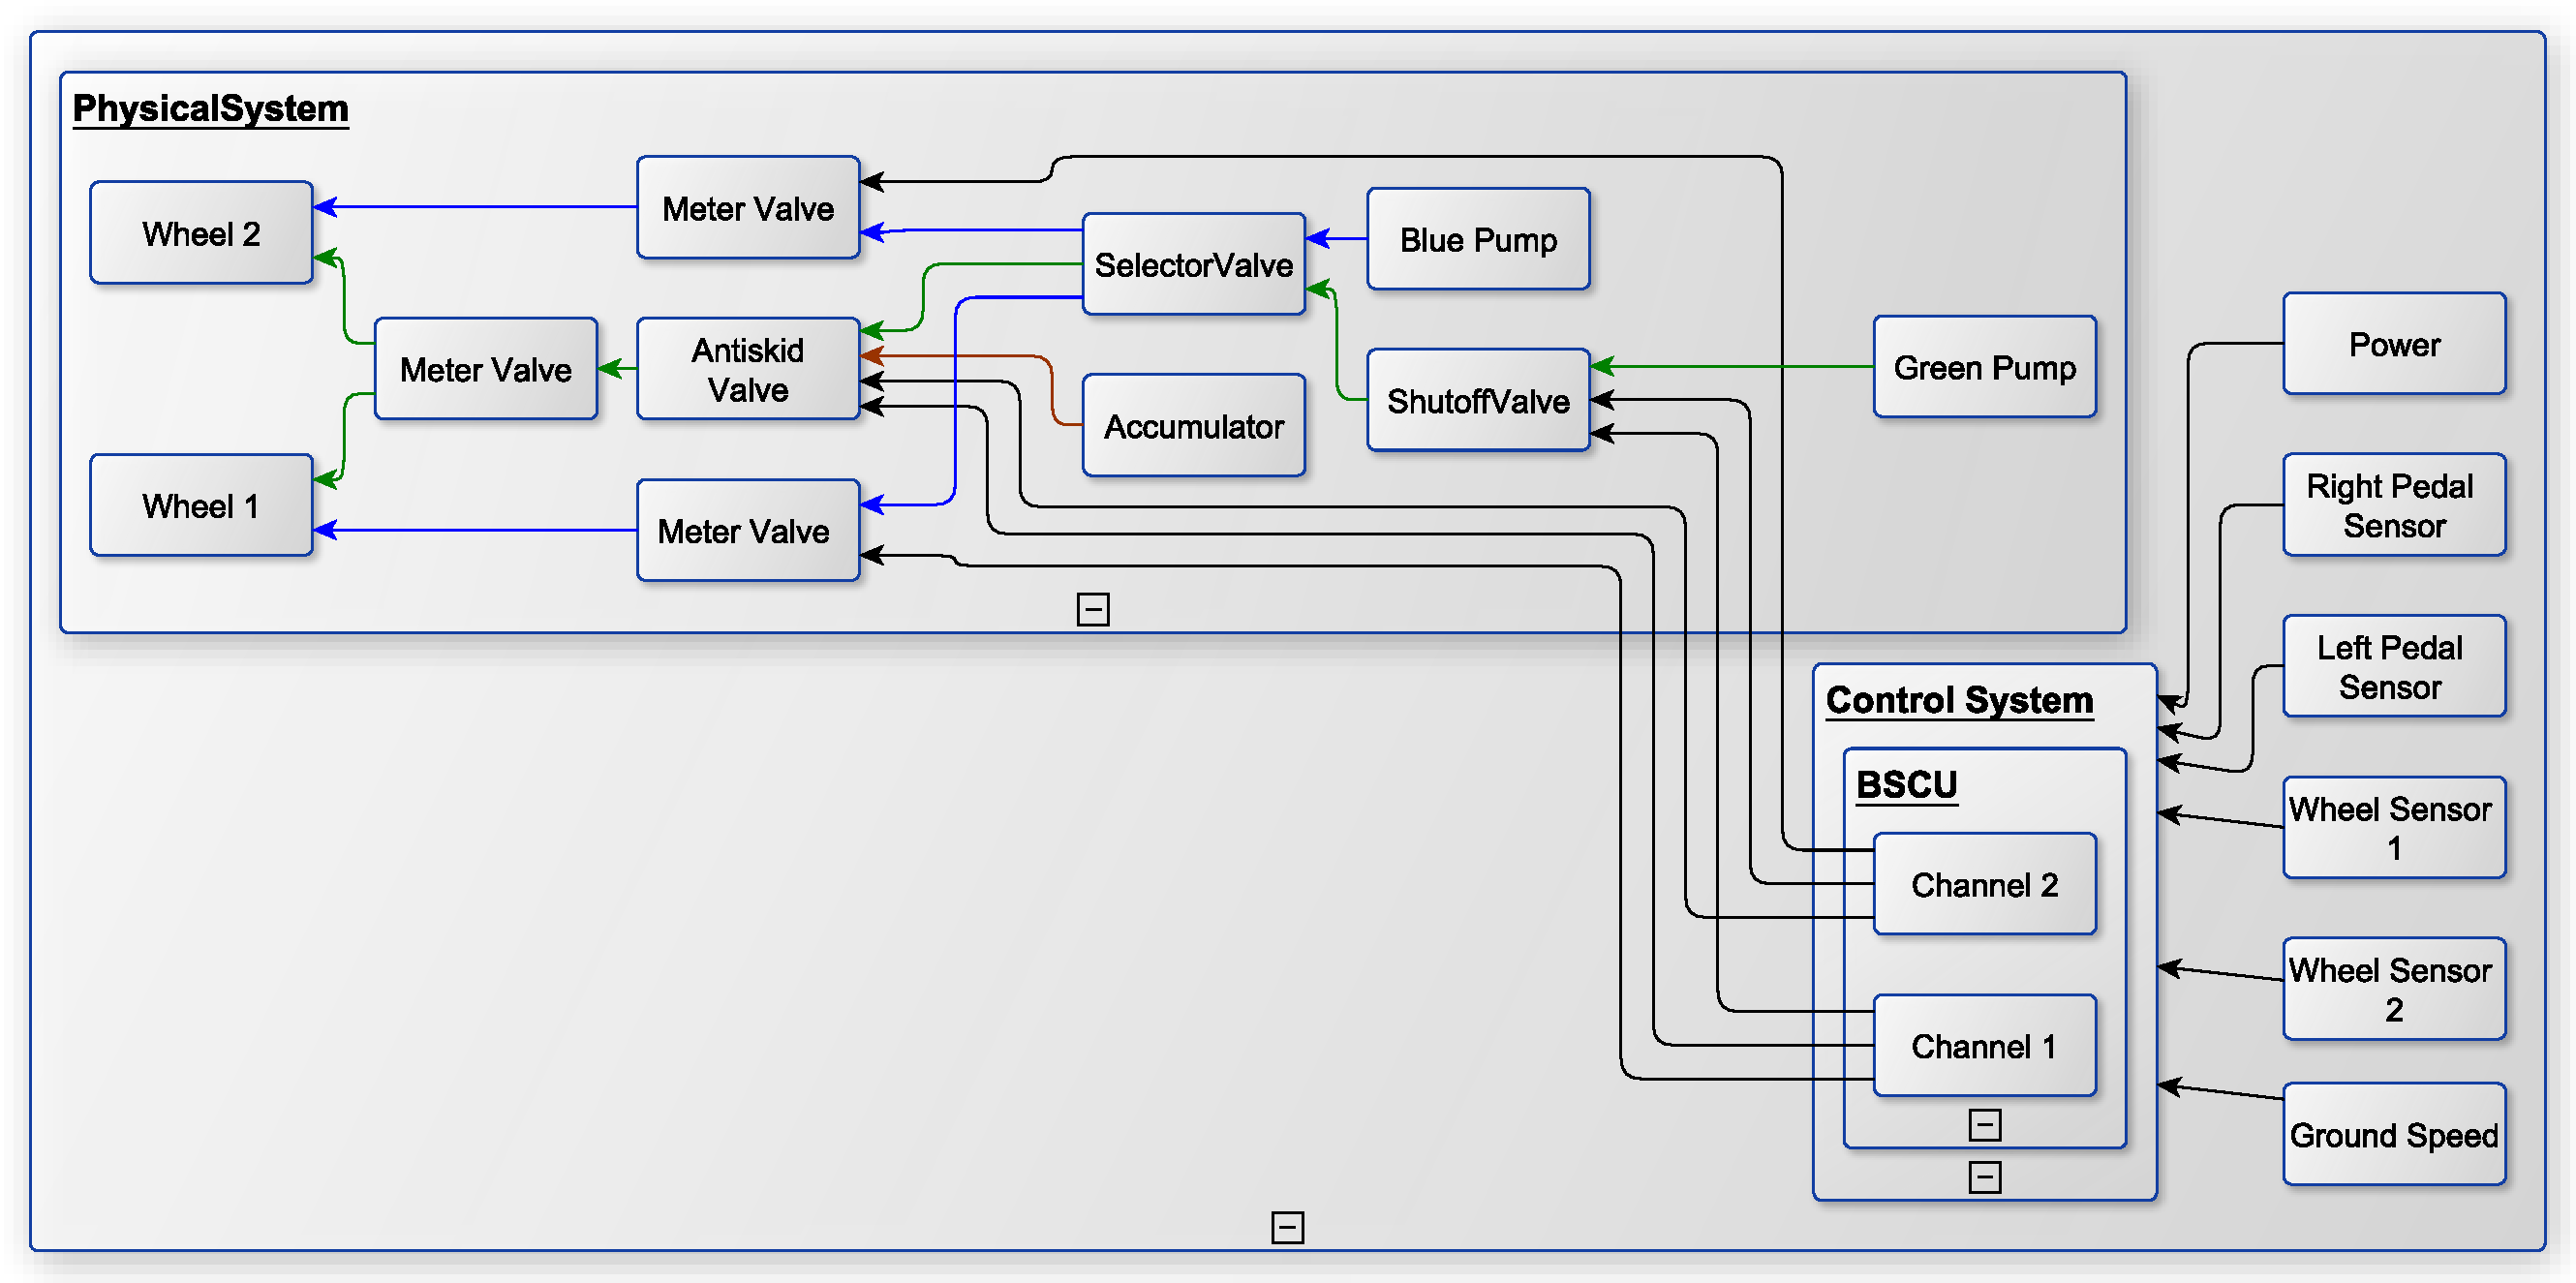
\includegraphics[trim=0 9 0 5,clip,width=\textwidth]{images/wbs_arch4_diagram.pdf}
	\caption{Wheel Brake System}
	\label{fig:wbs}
\end{figure} 

The WBS is composed of two main parts: the control system and the physical system. The control system electronically controls the physical system and contains a redundant channel of the Braking System Control Unit (BSCU) in case of failure. It also commands antiskid braking.% in case of skidding on the ground. 
The physical system consists of the hydraulic circuits running from hydraulic pumps to wheel brakes as well as valves that control the hydraulic fluid flow. This system provides braking force to each of the eight wheels of the aircraft. The wheels are all mechanically braked in pairs (one pair per landing gear). For simplicity, Figure~\ref{fig:wbs} displays only two of the eight wheels. 

There are three operating modes in the WBS model:

\begin{itemize}
	\renewcommand{\labelitemi}{\textbullet}
	\item In \textit{normal} mode, the system is composed of a \textit{green} hydraulic pump and one meter valve per each of the eight wheels. Each of the meter valves are controlled through electronic commands coming from the active channel of the BSCU. These signals provide braking and antiskid commands for each wheel. The braking command is determined through a sensor on the pedal and the antiskid command is determined by the \textit{Wheel Sensors}. 
	\item In \textit{alternate} mode, the system is composed of a \textit{blue} hydraulic pump, four meter valves, and four antiskid shutoff valves, one for each landing gear. The meter valves are mechanically commanded through the pilot pedal corresponding to each landing gear. If the system detects lack of pressure in the green circuit, the BSCU channel commands the selector valve to switch to the blue circuit. 
	\item In \textit{emergency} mode, the system mode is entered if the \textit{blue} hydraulic pump fails. The accumulator pump has a reserve of pressurized hydraulic fluid and will supply this to the blue circuit in emergency mode. 
\end{itemize}

The WBS architecture model in AADL contains 30 different kinds of components, 169 component instances, and a model depth of 5 hierarchical levels. 


%If the BSCU channel becomes invalid, the shutoff valve closes and we move into alternate mode. Once this system switches into alternate mode, it does not return to normal operation mode.

%There are three operating modes in the WBS model. In \textit{normal} mode, the system uses the \textit{green} hydraulic circuit. The normal system is composed of the green hydraulic pump and one meter valve per each of the eight wheels. Each of the meter valves are controlled through electronic commands coming from the active channel of the BSCU. These signals provide braking and antiskid commands for each wheel. The braking command is determined through a sensor on the pilot pedal position and is labeled as \textit{Left/Right Pedal Sensor} in Figure~\ref{fig:wbs} and the antiskid command is determined by the \textit{Wheel Sensors}. 

%In \textit{alternate} mode, the system uses the \textit{blue} hydraulic circuit. The alternate system is composed of the blue hydraulic pump, four meter valves, and four antiskid shutoff valves: one for each landing gear. The meter valves are mechanically commanded through the pilot pedal corresponding to each landing gear. If the system detects lack of pressure in the green circuit, the BSCU channel commands the selector valve to switch to the blue circuit. 
%If the BSCU channel becomes invalid, the shutoff valve closes and we move into alternate mode. Once this system switches into alternate mode, it does not return to normal operation mode.

%The last mode of operation of the WBS is the \textit{emergency} mode. This mode is entered if the blue hydraulic pump fails. The accumulator pump has a reserve of pressurized hydraulic fluid and will supply this to the blue circuit in emergency mode.

%The model contains 30 different kinds of components, 169 component instances, a model depth of 5 hierarchical levels.  The model includes one top-level assumption and  11 top-level system properties, with 113 guarantees allocated to subsystems.  There are a total of 33 different fault types and 141 fault instances within the model.  The large number of fault instances is due to the redundancy in the system design and its replication to control 8 wheels.

The behavioral model is encoded using the AGREE annex and the behavior is based on descriptions found in AIR6110. The top level system properties are given by the requirements and safety objectives in AIR6110. All of the subcomponent contracts support these system safety objectives through the use of assumptions on component input and guarantees on the output. The WBS behavioral model in AGREE annex includes one top-level assumption and  11 top-level system properties, with 113 guarantees allocated to subsystems.  

An example system safety property is to ensure that there is no inadvertent braking of any of the wheels. This is based on a failure condition described in AIR6110 is \textit{Inadvertent wheel braking on one wheel during takeoff shall be less than 1E-9 per takeoff}. 
Inadvertent braking means that braking force is applied at the wheel but the pilot has not pressed the brake pedal.  In addition, the inadvertent braking requires that power and hydraulic pressure are both present, the plane is not stopped, and the wheel is rolling (not skidding). This AGREE contract is shown \janet{below}. 
%in Figure~\ref{fig:inadvertent_braking}. 
The property is stated in AGREE such that inadvertent braking does \textit{not} occur.

\begin{figure}[h!]
	\vspace{-0.2in}
	\begin{center}
		\includegraphics[width=.8\textwidth]{images/inadvertent_braking.png}
	\end{center}
	\vspace{-0.3in}
	%\caption{AGREE Contract for Top Level Property}
	\label{fig:inadvertent_braking}
	\vspace{-0.2in}
\end{figure}


\subsection{Component Fault Modeling}

The usage of the terms error, failure, and fault are defined in ARP4754A and are described here for ease of understanding~\cite{SAE:ARP4754A}. An \textit{error} is a mistake made in implementation, design, or requirements. A \textit{fault} is the manifestation of an error and a \textit{failure} is an event that occurs when the delivered service of a system deviates from correct behavior. If a fault is activated under the right circumstances, that fault can lead to a failure. The terminology used in EMV2 differs slightly for an error: an error is a corrupted state caused by a fault. The error propagates through a system and can  manifest as a failure. In this paper, we use the ARP4754A terminology with the added definition of \textit{error propagation} as used in EMV2. An error is a mistake made in design or code and an error propagation is the corrupted state caused by an active fault. 

The Safety Annex is used to add potential faulty behaviors to a component model.  When the fault is activated by its specified triggering conditions, it modifies the output of the component. This faulty behavior may violate the contracts of other components in the system, including assumptions of downstream components. The impact of a fault is computed by the AGREE model checker when the safety analysis is run on the fault model. Examples of such faults include valves being stuck open or closed, output of a software component being nondeterministic, or power being cut off. 
%Faulty components can be mechanical or digital, but in this section we focus on a digital component in the WBS -- a brake pedal position sensor component. 

One of the components important to the inadvertent braking property is the brake pedal. When the mechanical pedal is pressed, a sensor reads this information and passes an electronic signal to the BSCU which then commands hydraulic pressure to the wheels. 

%Figure~\ref{fig:sensor} 
\janet{Below} shows the AADL pedal sensor component with a contract for its nominal behavior. The sensor has only one input, the mechanical pedal position, and one output, the electrical pedal position. %The 
\janet{A} property that governs the behavior of the component is that the mechanical position should always equal the electronic position. 

\begin{figure}[h!]
	\hspace*{-2cm}
	\vspace{-0.55in} 
	\begin{center}
		\includegraphics[trim=0 640 -10 70,clip,width=1.5\dimexpr\textwidth-2cm\relax]{images/system_sensor.pdf}
		\vspace{-0.3in}
	%	\caption{An AADL System Type: The Pedal Sensor}
		\label{fig:sensor}
	\end{center}
	\vspace{-0.4in}
\end{figure}

One possible failure for this sensor is inversion of its output value. This fault can be triggered with probability $5.0\times 10^{-6}$ as described in AIR6110 (in reality, the component failure probability is 
collected from hardware specification sheets).  %Figure~\ref{fig:sensorFault} 
\janet{Below} shows the Safety Annex definition for this fault. Fault behaviors may be defined by the user or by using a library of fault nodes, in this case, \textit{inverted\_fail}.  When the fault is triggered, the nominal output of the component (\textit{elec\_pedal\_position}) is replaced with its failure value (\textit{val\_out}). 

\begin{figure}[h!]
	\hspace*{-2cm}
	\vspace{-0.5in} 
	\begin{center}
		\includegraphics[trim=0 690 -10 70,clip,width=1.5\dimexpr\textwidth-2cm\relax]{images/safetyannex_sensorfault.pdf}
		\vspace{-0.3in}
		%\caption{The Safety Annex for the Pedal Sensor}
		\label{fig:sensorFault}
	\end{center}
	\vspace{-0.3in}
\end{figure}

The WBS fault model in Safety Annex contains a total of 33 different fault types and 141 fault instances. The large number of fault instances is due to the redundancy in the system design and its replication to control 8 wheels.

\subsection{Implicit %Failure
	\janet{Error} Propagation}
In the Safety Annex approach, faults are captured as faulty behaviors that augment the system behavioral model in AGREE contracts. No explicit %fault
\janet{error} propagation is necessary since the faulty behavior itself propagates through the system just as in the nominal system model. The effects of any triggered fault are manifested through analysis of the AGREE contracts. 

On the contrary, in the AADL Error Model Annex, Version 2 (EMV2)~\cite{EMV2} approach, all errors must be explicitly propagated through each component (by applying fault types on each of the output ports) in order for a component to have an impact on the rest of the system. To illustrate the key differences between implicit %failure
\janet{error} propagation provided in Safety Annex and the explicit %failure 
\janet{error} propagation provided in EMV2, we use a simplified behavioral flow from the WBS example using code fragments from EMV2, AGREE, and the Safety Annex. 

\begin{figure}[t]
	\vspace{-0.19in}
	\centering
	\includegraphics[trim=0 9 0 5,clip,width=\textwidth]{images/Comparison_with_EMV2.pdf}
	\vspace{-0.3in}
	\caption{Differences between Safety Annex and EMV2}
	\label{fig:comparison_with_EMV2}
	\vspace{-0.2in}
\end{figure} 

In this simplified WBS system, the physical signal from the Pedal component is detected by the Sensor and the pedal position value is passed to the Braking System Control Unit (BSCU) components.  The BSCU generates a pressure command to the Valve component which applies hydraulic brake pressure to the Wheels. 

In the EMV2 approach (top half of Figure~\ref{fig:comparison_with_EMV2}), the ``NoService'' fault is explicitly propagated through all of the components. These fault types are essentially tokens that do not capture any analyzable behavior. At the system level, analysis tools supporting the EMV2 annex can aggregate the propagation information from different components to compose an overall fault flow diagram or fault tree. 

When a fault is triggered in the Safety Annex (bottom half of Figure~\ref{fig:comparison_with_EMV2}), the output behavior of the Sensor component is modified. In this case the result is a ``stuck at zero'' error. The behavior of the BSCU receives a zero input and proceeds as if the pedal has not been pressed. This will cause the top level system contract to fail: {\em pedal pressed implies brake pressure output is positive}.

\begin{comment}
%\subsection{Comparison to the AADL Error Annex}

The AADL language has previously been extended to provide some fault modeling and analysis capabilities using its Error Model Annex, Version 2 (EMV2)~\cite{EMV2}.  EMV2 focuses on injection and propagation of discrete faults for generation of fault trees, rather than on analysis of system behavior in the presence of faults. 
To illustrate some of the key differences between our approach and the EMV2 approach, Figure~\ref{fig:comparison_with_EMV2} shows a simplified  behavioral flow with code fragments from EMV2, AGREE, and the Safety Annex. 

\begin{figure}[t]
	\vspace{-0.45in}
	\centering
	\includegraphics[trim=0 9 0 5,clip,width=\textwidth]{images/Comparison_with_EMV2.pdf}
	%\vspace{0.4in}
	\caption{Differences between Safety Annex and EMV2}
	\label{fig:comparison_with_EMV2}
\end{figure} 

In this simplified WBS system, the physical signal from the Pedal component is detected by the Sensor, and the pedal position value is passed to the Braking System Control Unit (BSCU) components.  The BSCU generates a pressure command to the Valve component which applies hydraulic brake pressure to the Wheels. 

In the EMV2 approach (top half of Figure~\ref{fig:comparison_with_EMV2}), all errors must be explicitly propagated through each component (by applying fault types on each of the output ports) in order for a component to have an impact on the rest of the system. In the example, the ``NoService'' fault is explicitly allowed by the EMV2 declarations to propagate through all of the components.  These fault types are essentially tokens that do not capture any analyzable behavior.  At the system level, analysis tools supporting the EMV2 annex can aggregate the fault flow and propagation information from different components to compose an overall fault flow diagram or fault tree.

In the Safety Annex approach (bottom half of Figure~\ref{fig:comparison_with_EMV2}), faults augment the system behavioral model through the AGREE contracts.  When a fault is triggered, the output behavior of the Sensor component is modified, in this case resulting a ``stuck at zero'' error. The behavior of the BSCU receives a zero input and proceeds as if the pedal has not been pressed. This will cause the top level system contract to fail: {\em pedal pressed implies brake pressure output is positive}. No explicit propagation is necessary since the faulty behavior propagates through the system just as in the nominal system model. The system and component failures are manifested through analysis of the AGREE contracts. 
\end{comment}

\subsection{Explicit %Failure 
	\janet{Error} Propagation} 
%Faults
\janet{Failures} in hardware (HW) components can trigger behavioral faults in the system components that depend on them. For example, a CPU %fault
\janet{Failure} may trigger faulty behavior in the threads bound to that CPU. In addition, a %fault
\janet{failure} in one HW component may trigger %faults
\janet{failure} in other HW components located nearby, such as overheating, fire, or explosion
in the containment location. 
The Safety Annex provides the capability to explicitly model the impact of hardware %faults
\janet{failures} on other faults, behavioral or non behavioral. The explicit propagation to non behavioral faults is similar to that provided in EMV2.

To better model %HW dependent faults 
\janet{faults at the system level dependent on HW failures}, a fault model element is introduced called a \janet{\textit{hardware fault}}. Users are not required to specify behavioral effects for the HW faults, nor are data ports necessary on which to apply the fault definition. An example of a model component fault declaration is shown \janet{below}:
\begin{figure}[h!]
	\vspace{-0.2in}
	\begin{center}
	\includegraphics[width=.7\textwidth]{images/hw_fault2.png}
	\end{center}
	\vspace{-0.3in}
	%\caption{Hardware Fault Definition}
	\label{fig:hwFault}
	%\vspace{-0.2in}
	\vspace{-0.1in}
\end{figure}

Users specify dependencies between the HW component faults and faults that are defined in other components, either HW or SW. The hardware fault then acts as a trigger for dependent faults. This allows a simple propagation from the faulty HW component to the SW components that rely on it, affecting the behavior on the outputs of the affected SW components.

%As an example, we will look yet again at the WBS. 
In the WBS example, assume that both the green and blue hydraulic pumps are located in the same compartment in the aircraft and an explosion in this compartment rendered both pumps inoperable.
%An accident took place and the green (normal) hydraulic pump took the force of an explosion. When the green hydraulic pump exploded, the pump shrapnel flew into the blue pump and it became from then on unoperable. 
The HW fault definition can be modeled first in the green hydraulic pump component as shown in Figure~\ref{fig:hwFault}. The activation of this fault triggers the activation of related faults as seen in the \textit{propagate\_to} statement shown \janet{below}. % in Figure~\ref{fig:hwFaultProp}. 
Notice that these pumps need not be connected through a data port in order to specify this propagation. %Furthermore, the probability of the HW fault activation can be specified. 

\begin{figure}[h!]
	\vspace{-0.2in}
	\begin{center}
		\includegraphics[width=1.0\textwidth]{images/hw_prop_stmt.png}
	\end{center}
	\vspace{-0.3in}
	%\caption{Hardware Fault Propagation Statement}
	\label{fig:hwFaultProp}
	%\vspace{-0.2in}
	\vspace{-0.1in}
\end{figure}

The fault dependencies are specified in the system implementation where the system configuration that causes the dependencies becomes clear (e.g., binding between SW and HW components, co-location of HW components). 
%This is because fault propagations are typically tied to the way components are connected or bound together; this information may not be available when faults are being specified for individual components. Having fault propagations specified outside of a component’s fault statements also makes it easier to reuse the component in different systems. 


\begin{comment}
\subsection{Fault Hypothesis}

An annotation in the AADL model determines the fault hypothesis. This may specify either a maximum number of faults that can be active at any point in execution (see Figure~\ref{fig:hwFaultProp}) or that only faults whose probability of simultaneous occurrence is above some probability threshold should be considered. Tying back to traditional safety analysis, the former is analogous to restricting the cutsets to a specified maximum number of terms, and the latter is analogous to restricting the cutsets to only those whose probability is above some set value.

In the former case, we assert that the sum of the true {\em fault\_\_trigger} variables is below some integer threshold.  In the latter, we determine all combinations of faults whose probabilities are above the specified probability threshold, and describe this as a proposition over {\em fault\_\_trigger} variables. 
%
With the introduction of dependent faults, active faults are divided into two categories: independently active (activated by its own triggering event) and dependently active (activated when the faults they depend on become active). The top level fault hypothesis applies to independently active faults. Faulty behaviors augment nominal behaviors whenever their corresponding faults are active (either independently active or dependently active).
\end{comment}










\section{Architecture and Implementation}
\label{sec:implementation}

The Safety Annex is written in Java as a plug-in for the OSATE AADL toolset, which is built on Eclipse.  It is not designed as a stand-alone extension of the language, but works with behavioral contracts specified in AGREE AADL annex~\cite{NFM2012:CoGaMiWhLaLu}. 
The architecture of the Safety Annex is shown in Figure~\ref{fig:plugin-arch}.

 %AGREE allows {\em assume-guarantee} behavioral contracts to be added to AADL components.  The language used for contract specification is based on the Lustre dataflow language~\cite{Halbwachs91:IEEE}. %AGREE improves scalability of formal verification to large systems by decomposing the analysis of a complex system architecture into a collection of smaller verification tasks that correspond to the structure of the architecture.

%\begin{comment}

\begin{figure}
	\begin{center}
		%\includegraphics[trim=0 400 430 0,clip,width=0.85\textwidth]{images/arch.png}
		\includegraphics[width=.9\textwidth]{images/arch.png}
	\end{center}
	\vspace{-0.2in}
	\caption{Safety Annex Plug-in Architecture}
	\label{fig:plugin-arch}
	\vspace{-0.2in}
\end{figure}

%\end{comment}

AGREE contracts are used to define the nominal behaviors of system components as {\em guarantees} that hold when {\em assumptions} about the values the component's environment are met.  The Safety Annex extends these contracts to allow faults to modify the behavior of component inputs and outputs. 
% To support these extensions, AGREE implements an Eclipse extension point interface that allows other plug-ins to modify the generated abstract syntax tree (AST) prior to its submission to the solver.  If the Safety Annex is enabled, these faults are added to the AGREE contract and, when triggered, override the nominal guarantees provided by the component.  
An example of a portion of an initial AGREE node and its extended contract is shown in Figure~\ref{fig:lustre}. The left column of the figure shows the nominal Lustre pump definition is shown with an AGREE contract on the output; and the right column shows the additional local variables for the fault (boxes 1 and 2), the assertion binding the fault value to the nominal value (boxes 3 and 4), and the fault node definition (box 5).

%In the left column of the figure, the nominal Lustre pump definition is shown with an AGREE contract on the output. In the right column, the additional local variables for the fault are seen in boxes 1 and 2, the assertion binding the fault value to the nominal value is seen in boxes 3 and 4, and the fault node definition is given in box 5. 

Once augmented with fault information, the AGREE model follows the standard translation path to the model checker JKind~\cite{2017arXiv171201222G}, an infinite-state model checker for safety properties.  The augmentation includes traceability information so that when counterexamples are displayed to users, the active faults for each component are visualized.

\begin{figure}[h!]
	\hspace*{-2cm}
	\vspace{-0.3in} 
	\begin{center}
		%\includegraphics[trim=0 690 -10 70,clip,width=1.5\dimexpr\textwidth-2cm\relax]{images/lustre.pdf}
		\includegraphics[scale=0.3]{images/lustre.jpg}
		%\caption{Nominal AGREE node and its extension with faults}
	\caption{Nominal AGREE Node and Extension with Faults}
		\label{fig:lustre}
	\end{center}
	\vspace{-0.3in}
\end{figure}

\begin{comment}
The architecture of the Safety Annex is shown in Figure~\ref{fig:plugin-arch}.  It is written in Java as a plug-in for the OSATE AADL toolset, which is built on Eclipse.  It is not designed as a stand-alone extension of the language, but works with behavioral contracts specified in AGREE AADL annex and associated tools~\cite{NFM2012:CoGaMiWhLaLu}.  AGREE allows {\em assume-guarantee} behavioral contracts to be added to AADL components.  The language used for contract specification is based on the Lustre dataflow language~\cite{Halbwachs91:IEEE}. AGREE improves scalability of formal verification to large systems by decomposing the analysis of a complex system architecture into a collection of smaller verification tasks that correspond to the structure of the architecture.

\begin{figure}
	\begin{center}
		%\includegraphics[trim=0 400 430 0,clip,width=0.85\textwidth]{images/arch.png}
		\includegraphics[width=.9\textwidth]{images/arch.png}
	\end{center}
	\vspace{-0.2in}
	\caption{Safety Annex Plug-in Architecture}
	\label{fig:plugin-arch}
\end{figure}

AGREE contracts are used to define the nominal behaviors of system components as {\em guarantees} that hold when {\em assumptions} about the values the component's environment are met.  The Safety Annex extends these contracts to allow faults to modify the behavior of component inputs and outputs.  To support these extensions, AGREE implements an Eclipse extension point interface that allows other plug-ins to modify the generated abstract syntax tree (AST) prior to its submission to the solver.  If the Safety Annex is enabled, these faults are added to the AGREE contract and, when triggered, override the nominal guarantees provided by the component.  

An example of a portion of an initial AGREE node and its extended contract is shown in Figure~\ref{fig:lustre}. 
In the left column of the figure, the nominal Lustre pump definition is shown with an AGREE contract on the output. In the right column, the additional local variables for the fault are seen in boxes 1 and 2, the assertion binding the fault value to the nominal value is seen in boxes 3 and 4, and the fault node definition is given in box 5. 

\begin{figure}[h!]
	\hspace*{-2cm}
	\vspace{-0.3in} 
	\begin{center}
		%\includegraphics[trim=0 690 -10 70,clip,width=1.5\dimexpr\textwidth-2cm\relax]{images/lustre.pdf}
		\includegraphics[scale=0.3]{images/lustre.jpg}
		\caption{Nominal AGREE node and its extension with faults}
		\label{fig:lustre}
	\end{center}
	\vspace{-0.3in}
\end{figure}


Once augmented with fault information, the AGREE model follows the standard translation path to the model checker JKind~\cite{2017arXiv171201222G}, an infinite-state model checker for safety properties.  The augmentation includes traceability information so that when counterexamples are displayed to users, the active faults for each component are visualized.

The architecture of the Safety Annex is shown in Figure~\ref{fig:plugin-arch}.  It is written in Java as a plug-in for the OSATE AADL toolset, which is built on Eclipse.  It is not designed as a stand-alone extension of the language, but works with behavioral contracts specified in AGREE AADL annex and associated tools~\cite{NFM2012:CoGaMiWhLaLu}.  AGREE allows {\em assume-guarantee} behavioral contracts to be added to AADL components.  The language used for contract specification is based on the Lustre dataflow language~\cite{Halbwachs91:IEEE}. AGREE improves scalability of formal verification to large systems by decomposing the analysis of a complex system architecture into a collection of smaller verification tasks that correspond to the structure of the architecture.

\begin{figure}
	\begin{center}
		%\includegraphics[trim=0 400 430 0,clip,width=0.85\textwidth]{images/arch.png}
		\includegraphics[width=.9\textwidth]{images/arch.png}
	\end{center}
	\vspace{-0.2in}
	\caption{Safety Annex Plug-in Architecture}
	\label{fig:plugin-arch}
\end{figure}

AGREE contracts are used to define the nominal behaviors of system components as {\em guarantees} that hold when {\em assumptions} about the values the component's environment are met.  The Safety Annex extends these contracts to allow faults to modify the behavior of component inputs and outputs.  To support these extensions, AGREE implements an Eclipse extension point interface that allows other plug-ins to modify the generated abstract syntax tree (AST) prior to its submission to the solver.  If the Safety Annex is enabled, these faults are added to the AGREE contract and, when triggered, override the nominal guarantees provided by the component.  

An example of a portion of an initial AGREE node and its extended contract is shown in Figure~\ref{fig:lustre}.  %The \texttt{\_\_fault} variables and declarations are added to allow the contract to override the nominal behavioral constraints (provided by guarantees) on outputs.  In the Lustre language, \texttt{assertion}s are constraints that are assumed to hold in the transition system. 
In the left column of the figure, the nominal Lustre pump definition is shown with an AGREE contract on the output. In the right column, the additional local variables for the fault are seen in boxes 1 and 2, the assertion binding the fault value to the nominal value is seen in boxes 3 and 4, and the fault node definition is given in box 5. 

%A  benefit of utilizing the AGREE behavioral annex is the ability to perform both monolithic and compositional analysis on the nominal model. AGREE allows {\em assume-guarantee} behavioral contracts to be added to AADL components.  The language used for contract specification is based on the Lustre dataflow language~\cite{Halbwachs91:IEEE} and the nominal model (AADL model annotated with AGREE contracts) is translated into Lustre before being sent to the JKind model checker for verification\cite{2017arXiv171201222G}. 

%When a user selects to run the fault analysis during verification, the AGREE contracts are automatically extended in Lustre in order to allow faults to modify the behavior of component outputs. These injections into the Lustre model are shown in Figure~\ref{fig:lustre}. 

\begin{figure}[h!]
	\hspace*{-2cm}
	\vspace{-0.3in} 
	\begin{center}
		%\includegraphics[trim=0 690 -10 70,clip,width=1.5\dimexpr\textwidth-2cm\relax]{images/lustre.pdf}
		\includegraphics[scale=0.3]{images/lustre.jpg}
		\caption{Nominal AGREE node and its extension with faults}
		\label{fig:lustre}
	\end{center}
	\vspace{-0.3in}
\end{figure}

\begin{comment}
\begin{figure}
	\vspace{-0.1in}
	%\includegraphics[trim=30 150 120 10,clip,width=\textwidth]{images/sample_code.png}
	\includegraphics[width=\textwidth]{images/sample_code.png}
	\vspace{-0.3in}
	\caption{Nominal AGREE node and its extension with faults}
	\label{fig:comp}
\end{figure}
\end{comment}
%An annotation in the AADL model determines the fault hypothesis.  This may specify either a maximum number of faults that can be active at any point in execution (typically one or two), or that only faults whose probability of simultaneous occurrence is above some probability threshold should be considered. In the former case, we assert that the sum of the true {\em fault\_\_trigger} variables is below some integer threshold.  In the latter, we determine all combinations of faults whose probabilities are above the specified probability threshold, and describe this as a proposition over {\em fault\_\_trigger} variables.
%
%With the introduction of dependent faults, active faults are divided into two categories: independently active (activated by its own triggering event) and dependently active (activated when the faults they depend on become active). The top level fault hypothesis applies to independently active faults. Faulty behaviors augment nominal behaviors whenever their corresponding faults are active (either independently active or dependently active).

%Once augmented with fault information, the AGREE model follows the standard translation path to the model checker JKind~\cite{2017arXiv171201222G}, an infinite-state model checker for safety properties.  The augmentation includes traceability information so that when counterexamples are displayed to users, the active faults for each component are visualized.


%For fault analysis, we separate the possible analyses available to users into two distinct actions and describe them here.


\section{Analysis of the Fault Model}
\label{sec:fault_analysis}

When the Safety Annex is enabled, users can invoke either the monolithic analysis or compositional analysis in AGREE to check if the top level safety properties of the system hold in the presence of faults under the fault hypothesis given for the system. If an active fault causes the violation of a contract, a counterexample is provided by the model checker. The counterexample can be used to further analyze the system design and make necessary updates to the shared model between safety assessment and system development processes. This iterations continues until the system safety property is satisfied with the desired fault tolerance and failure probability achieved.

\subsection{Fault Hypothesis}
As the number of component faults increases, the different fault combinations can grow exponentially, making model checking infeasible. Therefore, a fault hypothesis needs to be specified for the system under verification to limit the simultaneous fault activations that are considered by the model checker.

A Safety Annex annotation in the system implementation of the AADL model determines the fault hypothesis. There are two types of fault hypothesis:

The \textit{max fault hypothesis} specifies a maximum number of faults that can be active at any point in execution. This is analogous to restricting the cutsets to a specified maximum number of terms in \janet{the fault tree analysis in}
traditional safety analysis. In implementation (i.e., the translated Lustre model feeding into the model checker), we assert that the sum of the true {\em fault\_\_trigger} variables is below some integer threshold. Each layer of the model needs to have a max fault hypothesis statement specified in order to consider fault activation in that layer in the analysis.

The \textit{probabilistic fault hypothesis} specifies that only faults whose probability of simultaneous occurrence is above some probability threshold should be considered (see Figure~\ref{fig:hwFaultProp}). This is analogous to restricting the cutsets to only those whose probability is above some set value. In implementation, we determine all combinations of faults whose probabilities are above the specified probability threshold and describe this as a proposition over {\em fault\_\_trigger} variables. Each subcomponent fault needs to specify a probability of occurrence in order to be considered in the analysis.

With the introduction of dependent faults, active faults are divided into two categories: independently active (activated by its own triggering event) and dependently active (activated when the faults they depend on become active). The top level fault hypothesis applies to independently active faults. Faulty behaviors augment nominal behaviors whenever their corresponding faults are active (either independently active or dependently active).

\subsection{Monolithic Analysis}
When monolithic analysis is performed on the nominal system model, the architectural model is flattened in order to perform the analysis. All of the contracts in the lower levels are used for the analysis.
%A top level threshold is defined within the safety annex located in the top level system implementation. In the lower levels, each defined subcomponent fault is given a probability of occurrence. 

Given a probabilistic fault hypothesis, this corresponds to performing a %prior 
analysis on which combinations of faults have a probability less than the threshold and then inserting assertions into the Lustre code accordingly. If the probability of such combination of faults is in fact less than the designated top level threshold, these faults may be activated and the behavioral effects can be seen through a counterexample.  

To perform this analysis, it is assumed that the non-hardware faults occur independently and possible combinations of faults are computed and passed to the Lustre model to be checked by the model checker. As seen in Algorithm 1, the computation first removes all faults from consideration that are too unlikely given the probability threshold. The remaining faults are arranged in a priority queue $\mathcal{Q}$ from high to low. Assuming independence in the set of faults, we take a fault with highest probability from the queue (step 5) and attempt to combine the remainder of the faults in $\mathcal{R}$ (step 7). If this combination is lower than the threshold (step 8), then we do not take into consideration this set of faults and instead remove the tail of the remaining faults in $\mathcal{R}$. %The reason we can do this is because of the arrangement in priority queue from highest to lowest value. If this combination is below threshold, certainly any other combination of these faults with one of lesser value in the priority queue will also be below threshold. 
 
In this calculation, we assume independence among the faults, but in the Safety Annex it is possible to define dependence between faults using a %\textit{hardware fault} node\
\janet{fault propagation statement}. After fault combinations are computed using Algorithm 1, the triggered dependent HW faults are added to the combination as appropriate. 

\begin{algorithm}[H]
	% \KwData{this text}
	% \KwResult{how to write algorithm with \LaTeX2e }
	$\mathcal{F} = \{\}$ : fault combinations above threshold \;
	$\mathcal{Q}$ : faults, $q_i$, arranged with probability high to low \;
	$\mathcal{R} = \mathcal{Q}$ , with $r \in \mathcal{R}$\;
	\While{$\mathcal{Q} \neq \{\} \land \mathcal{R} \neq \{\}$ }{
		$q =$ removePriorityElement($\mathcal{Q}$) \;
		\For{$i=0:|\mathcal{R}|$}{
			$prob = q \times r_i$ \;
			\eIf{prob $<$ threshold}{
				removeTail($\mathcal{R}, j=i:|\mathcal{R}|$)\;
			}{
				add($\{q, r_i\}, \mathcal{Q}$)\;
				add($\{q, r_i\}, \mathcal{F}$)\;
			} % end if else
		} % end for
	} % end while
	\caption{Monolithic Probability Analysis}
\end{algorithm}

%After all possible fault combinations are computed from Algorithm 1, we look at the collection of propagation statements used in HW fault definitions and add additional faults into the possible fault combinations if a fault that triggers the fault can become active, as computed from Algorithm 1.

%At the end of Algorithm 1, the possible fault combinations reside in the list $\mathcal{F}$. We then look at the collection of propagation statements used in HW fault definitions. These have a source (HW fault) and destination (faults triggered by HW fault). 

%Let $\mathcal{P}$ be the collection of propagation statements. For all $S \subset \mathcal{F}$, check to see if for $f \in S$, $f \in \mathcal{P}$ as a source. If so, add the corresponding destinations to the set $S$. This set $\mathcal{F}$ of allowed fault combinations is then added as a constraint to the Lustre model and thus they become active. If an active fault causes the violation of a contract, this is seen in a counterexample provided by the model checker.

\subsection{Compositional Analysis}
In compositional analysis, the analysis proceeds in a top down fashion. To prove the top level properties, the properties in the layer directly beneath the top level are used to perform the proof. The analysis proceeds in this manner.

The compositional analysis currently works with the max fault hypothesis. Users can constrain the maximum number of faults within each layer of the model by specifying the maximum fault hypothesis statement to that layer. If any lower level property failed due to activation of faults, the property verification at the higher level can no longer be trusted because the higher level properties were proved based on the assumption that the direct sublevel contracts are valid.

The compositional analysis is helpful to see weaknesses in a given 
layer of the system. In future work, we plan to reflect lower layer
property violations in the verification results of higher layers in the architecture and enable the display or constraint active faults system wide instead of layer wide.


%\subsection{Analysis Results of the WBS Example}
\subsection{Analysis of the WBS Example}
\label{sec:results}

The fault analysis on the top level WBS system was performed on the 11 top-level properties applying the max fault hypothesis and probabilistic fault hypothesis separately. It requires between 2 and 4 minutes to run either compositional analysis with max fault hypothesis or monolithic analysis with probabilistic fault hypothesis on the model. The analysis is computationally inexpensive, allowing quick iterations between systems and safety engineers.

We first applied compositional analysis with max one fault hypothesis at all layers of the model. Most properties were verified except for the \textit{Inadvertent braking at the wheel} properties. The failure of the verification for those properties shows that they are not resilient to a single fault. We then applied monolithic analysis with probabilistic fault hypothesis of $10^{-9}$ fault threshold. The \textit{Inadvertent braking at the wheel} properties \janet{also} failed. Results from the first round of checks indicate that the WBS design is not fault tolerant to the inadvertent braking properties and is not meeting the reliability goals of $10^{-9}$ on those properties.

The counterexample returned by the tools allowed us to straightforwardly diagnose the fault conditions that lead to property failure: in this model, there is a single pedal position sensor for the brake pedal. If this sensor fails, it can command braking without a pilot request. The counterexample can be used to further analyze the system design and explore a solution to the problem. There are several ways to proceed (here we note that the architecture of the pedal assembly is not discussed in AIR6110):
	\begin{itemize}
	\renewcommand{\labelitemi}{\textbullet}
	\item Increase the reliability of the brake pedal sensor. The failure probabilities are estimated from the failure rates and exposure times of the events. We may adjust the exposure time to match the phase of flight, rather than normalizing it per-flight-hour, if the phase of flight is sufficiently short. We may also find a brake pedal sensor with a lower failure rate. For example, if the failure probability for the sensor component is lower than the $10^{-9}$ fault threshold, it will not be considered in the possible fault combinations for the analysis. Increasing the reliability of the components could help increase the reliability of the system. However, the system still has a single point of failure in this case.
	
	\item Create redundancy in the sensor component and model a voting procedure.
	In order for braking to occur, both (or all) sensors must agree. This would eliminate a single point of failure and would also cause the model to meet the top level probabilistic threshold. However, by introducing redundancy, it could affect the probability of meeting of other properties in the system that command braking, for example, when braking is commanded, braking pressure is provided at the wheel. Introducing the redundancy can increase the reliability on inadvertent braking, but decrease the reliability on braking when needed.
\end{itemize}

Providing a way to quickly and effectively run analysis on the model %so that 
\janet{for} these different modes of failure can be of great benefit to assist system engineers to make design decisions and safety engineers to assess the effect.

\begin{comment}
The fault analysis on the top level WBS system was performed on the 11 top-level properties \janet{applying the max fault hypothesis and probabilistic fault hypothesis separately. It requires between 2 and 4 minutes to run either compositional analysis with max fault hypothesis or monolithic analysis with probabilistic fault hypothesis on the model. The analysis is computationally inexpensive, allowing quick iterations between systems and safety engineers.}

\janet{We first applied compositional analysis with max one fault hypothesis at all layers of the model.} Most properties were verified except for the \textit{Inadvertent braking at the wheel} properties. \janet{The failure of the verification for those properties shows that they are not resilient to a single fault.} The {\em counterexample} returned by the tools allowed us to straightforwardly diagnose the fault conditions that lead to property failure: In this model, there is a single pedal position sensor for the brake pedal. If this sensor fails, it can command braking without a pilot request.

This counterexample can be used to further analyze the system design.  For our model, there are several possible reasons for failure: it could be that redundant sensors are required on the pedals (here we note that the architecture of the pedal assembly is not discussed in AIR6110) or that the phase of flight is sufficiently short that we need to adjust our pedal failure rate to match this phase of flight, rather than normalizing the failure rate to per-flight-hour.  

\janet{We then applied monolithic analysis with probabilistic fault hypothesis of $10^{-9}$ fault threshold. The \textit{Inadvertent braking at the wheel} properties failed. Updating the probability of occurrence for the sensor components identified above to be above the fault threshold allowed the properties to pass, showing that increasing the reliability of those components help increase the reliability of the system.}

\danielle{Given these results, we were faced with a couple of options regarding the model. In order to meet the probabilistic threshold, one option is to find a brake pedal sensor with better reliability. Given that our top level threshold is $10^{-9}$, the sensor reliability must be less than this value. This is most likely an unrealistic solution, but even if it was possible, the model still has a single point of failure. This is shown thorugh the compositional analysis. The other option is to create redundancy in the sensor component and model a voting procedure. In order for braking to occur, both (or all) sensors must agree. This would eliminate a single point of failure and would also cause the model to meet the top level probabilistic threshold. The problem this raises is the complementary property in the system which states that when braking is commanded, braking pressure is provided at the wheel. By introducing redundancy, this also introduces a tradeoff between false positives and false negatives and directly affects the property regarding commanded braking.}

\danielle{These are realistic scenarios and decisions that are faced by system and safety engineers. Providing a way to quickly and effectively run analysis on the model so that these different modes of failure can be easily seen is of great benefit.} 


%It is computationally inexpensive to run the analysis, allowing quick iterations between systems and safety engineers. In the case of the WBS, it requires between 2 and 4 minutes to run either compositional (restricting the number of faults) or monolithic (probabilistic) fault analysis on the model.

%During our analysis, we discovered that most properties were verified, but the \textit{Inadvertent braking at the wheel} properties are not resilient to a single fault nor do they meet the desired $10^{-9}$ fault threshold for probabilistic analysis. In this model, there is a single pedal position sensor for the brake pedal.  If this sensor fails, it can command braking without a pilot request.  Given the {\em counterexample} returned by the tools, it is straightforward to diagnose the fault conditions that lead to property failure.


%what did we do monolithic, what did we do compositional
%what did we use max one fault
%what did we do with what probability


%The sync and update between the safety analysis artifacts and the system architecture/analysis model continues until the system safety property is satisfied with the desired fault tolerance and failure probability achieved.
\end{comment}

\begin{comment}

Fault analysis on the top level WBS system was performed on the 11 top-level properties using two fault hypotheses.  In the first case, we allow at most one fault, and in the second we allow combinations of faults that exceed the acceptable probability for the top-level hazard defined in AIR6110.

We use this model to demonstrate the benefits of formal fault analysis and to show the scalability of our tools.  We applied both monolithic and compositional analysis.

%\janet{Janet Note: TODO: replace timing data on something about what we learned from the analysis results, and use it to feedback to the system design, and rerun the analysis. As Mats pointed out, "can we add a redundant sensor and get fault tolerance?}
%\danielle{Danielle Note: The last 2 paragraphs of this section addresses this idea a little bit. One thing we can do is add a redundant sensor to the wbs model and run it to see what happens. If we do not want to add more to the model and perform analysis, then perhaps the last paragraphs of this section is good enough.}

%For the fault-free ``nominal'' system model, monolithic analysis requires 21 seconds, whereas compositional analysis requires 1 minute and 53 seconds.  Although the compositional time is longer, each sub-problem completes in less than 5 seconds.  The additional time for compositional analysis is  due to the start-up overhead to invoke the JKind model checker many times for individual layers.  On the other hand, when examining the model under a single-fault hypothesis, compositional analysis requires 2 minutes 6 seconds, while monolithic analysis did not terminate after 60 minutes.

%For probabilistic fault hypotheses, we are currently developing a sound approach for composition with respect to the top-level fault probability, but our current tool requires monolithic analysis.  In this case, given a probabilistic fault hypothesis of $5\times 10^{-7}$, monolithic analysis requires 3 minutes 25 seconds.

During our analysis, we discovered that most properties were verified, but the \textit{Inadvertent braking at the wheel} properties are not resilient to a single fault nor do they meet the desired $10^{-9}$ fault threshold for probabilistic analysis.  In this model, there is a single pedal position sensor for the brake pedal.  If this sensor fails, it can command braking without a pilot request.  Given the {\em counterexample} returned by the tools, it is straightforward to diagnose the fault conditions that lead to property failure.

This counterexample can be used to further analyze the system design.  For our model, there are several possible reasons for failure: it could be that redundant sensors are required on the pedals (here we note that the architecture of the pedal assembly is not discussed in AIR6110) or that the phase of flight is sufficiently short that we need to adjust our pedal failure rate to match this phase of flight, rather than normalizing the failure rate to per-flight-hour.  

It is computationally inexpensive to run the analysis, allowing quick iterations between systems and safety engineers. 
In the case of the WBS, it requires between 2 and 4 minutes to run either compositional (restricting the number of faults) or monolithic (probabilistic) fault analysis on the model.
The sync and update between the safety analysis artifacts and the system architecture/analysis model continues until the system safety property is satisfied with the desired fault tolerance and failure probability achieved.
\end{comment}

\section{Related Work}
\label{sec:related_work}

Formal model based systems engineering (MBSE) methods and tools now permit system level requirements to be specified and analyzed early in the development process~\cite{QFCS15:backes,CIMATTI2015333, NFM2012:CoGaMiWhLaLu, hilt2013:MuWhRaHe}. Design models from which aircraft systems are developed can be integrated into the safety analysis process to help guarantee accurate and consistent results. Integration of MBSA into safety analysis process is described by Bozzano and Villafiorita~\cite{Bozzano:2010:DSA:1951720}. There are tools that currently support reasoning about faults in architecture description languages such as SysML and AADL. We provide here a brief overview of the most relevant safety analysis tools. 

Tools such as the AADL Error Model Annex, Version 2 (EMV2)~\cite{EMV2} and HiP-HOPS for EAST-ADL~\cite{CHEN201391} primarily utilize \textit{qualitative} reasoning. Faults are enumerated and the propagations through system components are explicitly described. Given many possible faults, these propagation relationships increase in complexity and understandability. Interactions are easily overlooked by analysts and thus not explicitly described. In our approach, faults are injected into the system and behaviorally propagated through the use of assume-guarantee statements in AGREE. This avoids the difficulties inherent with explicit fault enumeration and propagation. 

% Say something about behavioral propagation here ---------------------------------------------------

SmartIFlow~\cite{info8010007} is a purpose-built safety analysis tool that describes components and their interactions using finite state machines and events. Verification is done through an explicit state model checker which returns sets of counterexamples for safety requirements in the face of failures. The mechanism to keep the search space size under control during model checking relies on expert knowledge from engineers. This limits the number of failures and removes the possibility of certain failure conditions. Due to this drawback, scalability to industrial sized systems is difficult. The safety annex described in this research is not a standalone model, but is made to be incorporated into the system safety assessment process as described in section 2.1. \danielle{Scalability: in terms of the safety annex, just reference the case study described in this work?}

Another approach has been introduced by G{\"u}demann et. al.~\cite{Gudemann:2010:FQQ:1909626.1909813}. System models are constructed in SAML (Safety Analysis and Modeling Language) which can be imported into several analysis tools like NuSMV~\cite{Cimatti2000} or PRISM~\cite{CAV2011:KwNoPa} (Probabilistic Symbolic Model Checker) or MRMC probabilistic model checker~\cite{Katoen:2005:MRM:1114692.1115230}. SAML is used for both qualitative and quantitative analyses and allows for the combination of discrete probability distributions and non-determinism. The framework is used to create a system model comprised of software control, hardware components, environment and failure mode modeling. 

In earlier work, an approach to MBSA was demonstrated using the Simulink\textsuperscript{\textregistered} notation~\cite{Joshi05:SafeComp,Joshi05:Dasc}. In this approach, a behavioral model of system dynamics was used to reason about the effects of faults in the system. This approach allows an implicit and natural notion of fault propagation through the system. However, non-functional architectural properties were not captured as Simulink is not designed as an architecture description language. In our approach, we are applying quantitative reasoning and implicit fault propagation to a more rich architecture language.

Similarly, AltaRica~\cite{PROSVIRNOVA2013127} has been incorporated into Cecilia OCAS as a model based safety analysis tool~\cite{BieberERTS2018}. Safety assessment, fault tree generation, and functional verification can be performed with the aid of NuSMV model checking~\cite{symbAltaRica}. Failure states are defined throughout the system and flow variables are updated through the use of assertions~\cite{Bieber04safetyassessment}. A limitation of this is that Linear Temporal Logic operators are required in some of the failure definitions. This is a downfall to the safety community/engineers who are not familiar with LTL~\cite{Bieber04safetyassessment}. 

Closely related to our work is the model-based safety assessment toolset called COMPASS (Correctness, Modeling project and Performance of Aerospace Systems)~\cite{10.1007/978-3-642-04468-7_15}. COMPASS uses the SLIM language which is based on AADL, for its input models. The SLIM (System Level Integrated Modeling Language) language was developed by the COMPASS project for modeling hardware and software systems for safety-related tasks~\cite{5185388, criticalembeddedsystems}. System models in SLIM are translated into the input language of NuSMV and xSAP~\cite{DBLP:conf/tacas/BittnerBCCGGMMZ16} is invoked to generate safety analysis artifacts (e.g. Fault Trees, FMEA tables, etc.)~\cite{compass30toolset}.

Formal verification tools based on model checking have been used to automate the generation of safety artifacts~\cite{symbAltaRica,10.1007/978-3-540-75596-8-13, DBLP:conf/tacas/BittnerBCCGGMMZ16}. This approach has limitations in terms of scalability and readability of the fault trees generated. Work has been done towards mitigating these limitations by the scalable generation of readable fault trees~\cite{10.1007/978-3-319-11936-6-7}.



\section{Conclusions \& Future Work}
In this paper, we describe our initial work towards performing MBSA using the AADL architecture description language using a failure effect modeling approach.  Our goal is to be able to perform safety analysis on common models used by systems and safety engineers for functional and non-functional analyses, schedulability, and perhaps system image generation.  To perform this analysis, we use existing capabilities within AADL to describe the structure of the system, and build on the existing AGREE framework for compositional analysis of components.  

As part of our exploration, we are interested in examining the strengths and weaknesses of our FEM and the AADL Error Annex FLM-based approach.  We believe that the FEM approach has advantages both in terms of brevity of specifications and accuracy of results, and can build on existing analyses performed for systems engineering.  However, there are also risks in the FEM approach involving incomplete or mis-specified properties.  

We illustrated the ideas using architecture models based on the Wheel Braking System model in SAE AIR 6110 \cite{AIR6110} and use this in the evaluation of our approach. Using assume-guarantee compositional reasoning techniques, we prove a top level property of the wheel brake system that states when the brake pedals are pressed in the absence of skidding, there will be hydraulic pressure supplied to the brakes.  

Starting from the error model notions of error types, two main faults were defined: \textit{fail\_to} which will describe failures of valves and pressure regulators and \textit{inverted\_fail} which describes the failures occurring to components that output boolean values. Using the AADL behavioral model of the WBS, these permanent faults were tied into the nominal model in order to reason about how this model behaves in the presence of specific kinds of faults.

In order to demonstrate that the system was resilient to single faults, we modified the model to allow feedback from the wheel pressure to the BSCU.   This changed the way the system responded to faults that were further downstream of the BSCU or Selector and created a chance for the system to switch to alternate forms of hydraulic pressure. We also reasoned about the initialization values of the system in regards to which mode is the starting mode. It is crucial for the system to begin in Normal mode in order to function successfully in the presence of faults.  After model modification and a small weakening of our original property to account for feedback delay, the model does fulfill the top level contract even when a permanent fault of one of the high level components is introduced.

The current capabilities of AGREE are well-suited to specifying faults.  Our approach allows for scalar types of unbounded integers and reals, as well as composite types such as tuples and structures.  It is possible to model systems and reason about them in either discrete time or real-time.  However, adding faults to existing components is cumbersome and can obscure the nominal behaviors of the model.  We are currently examining several fault specification languages, giving special consideration to the xSAP modeling language.

Future research work will involve the continuation of development of the methods and tools needed to perform model-based safety analysis at the system architecture level. By introducing a common set of models for both nominal system design and safety analysis, we hope to reduce the cost of development and improve safety. Our hope is to demonstrate the practicality of formal analysis for early detection of safety issues that would be prohibitively expensive to find through testing and inspection. We will base this research on industry standard notations that are being used in airborne and ground-based avionics in order to ensure transition of this technology.

\subsection*{Acknowledgements} This research was funded by NASA AMASE NNL16AB07T and University of Minnesota College of Science and Engineering Graduate Fellowship.




\vspace{-0.40cm}
\bibliographystyle{abbrv}
\bibliography{biblio}
%\vspace{-7.25cm}
% This ~ seems to fix an odd bibliography alignment issue
~

%\ifdefined\TECHREPORT
%\appendix
%
%\section{Appendix: Proof of Equivalence}
%\input{appendix}
%\fi

%\section{Appendix: GPCA CENTA Model}
%\label{appendix:gpcacenta}
%\begin{figure}[!ht]
%\begin{center}
%\includegraphics[scale=0.6]{images/sampled_pca.PNG} %[trim = 0 2 0 0, clip=true]{Comp}
%\caption{GPCA AGREE Properties modeled as a Timed Automata} \label{fig:samplepca}
%\end{center}
%\end{figure}

%\balancecolumns

\end{document} 